\documentclass[]{default}
\usepackage{lmodern}
\usepackage{listings}
\usepackage{amssymb,amsmath}
\usepackage{paralist}
\usepackage{tikz-qtree}
\usepackage{enumitem}
\usepackage{ifxetex,ifluatex}
\usepackage{fixltx2e} % provides \textsubscript
\ifnum0\ifxetex{1}\fi\ifluatex{1}\fi=0 % if pdftex
  \usepackage[T1]{fontenc}
  \usepackage[utf8]{inputenc}
\else % if luatex or xelatex
  \ifxetex{
    \usepackage{mathspec}
    \usepackage{xltxtra,xunicode}
  \else
    \usepackage{fontspec}
  }\fi
  \defaultfontfeatures{Mapping=tex-text,Scale=MatchLowercase}
  \newcommand{\euro}{€}
\fi
% use upquote if available, for straight quotes in verbatim environments
\IfFileExists{upquote.sty}{\usepackage{upquote}}{}
% use microtype if available
\IfFileExists{microtype.sty}{%
\usepackage{microtype}
\UseMicrotypeSet[protrusion]{basicmath} % disable protrusion for tt fonts
}{}
\ifxetex%
  \usepackage[setpagesize=false, % page size defined by xetex
              unicode=false, % unicode breaks when used with xetex
              xetex]{hyperref}
\else
  \usepackage[unicode=true]{hyperref}
\fi
\hypersetup{breaklinks=true,
            bookmarks=true,
            pdfauthor={},
            pdftitle={Quantitative Benchmarks for Theory Exploration},
            colorlinks=true,
            citecolor=blue,
            urlcolor=blue,
            linkcolor=magenta,
            pdfborder={0 0 0}}
\urlstyle{same}  % don't use monospace font for urls
\setlength{\parindent}{0pt}
\setlength{\parskip}{6pt plus 2pt minus 1pt}
\setlength{\emergencystretch}{3em}  % prevent overfull lines
\setcounter{secnumdepth}{5}

\newcommand{\name}[1]{\mathrm{#1}}

\newcommand{\feature}[1]{\phi(#1)}
\newcommand{\id}[1]{\texttt{``#1''}}
\newcommand{\CVar}{\texttt{Var}}
\newcommand{\CLit}{\texttt{Lit}}
\newcommand{\CApp}{\texttt{App}}
\newcommand{\CLam}{\texttt{Lam}}
\newcommand{\CLet}{\texttt{Let}}
\newcommand{\CCase}{\texttt{Case}}
\newcommand{\CType}{\texttt{Type}}
\newcommand{\CLocal}{\texttt{Local}}
\newcommand{\CGlobal}{\texttt{Global}}
\newcommand{\CConstructor}{\texttt{Constructor}}
\newcommand{\CLitNum}{\texttt{LitNum}}
\newcommand{\CLitStr}{\texttt{LitStr}}
\newcommand{\CAlt}{\texttt{Alt}}
\newcommand{\CDataAlt}{\texttt{DataAlt}}
\newcommand{\CLitAlt}{\texttt{LitAlt}}
\newcommand{\CDefault}{\texttt{Default}}
\newcommand{\CNonRec}{\texttt{NonRec}}
\newcommand{\CRec}{\texttt{Rec}}
\newcommand{\CBind}{\texttt{Bind}}

\newlist{inlinelist}{enumerate*}{1}
\setlist*[inlinelist,1]{%
  label= (\roman*),
}

\title{Quantitative Benchmarks for Theory Exploration}
  \author{Chris Warburton \\
          University of Dundee \\
          \texttt{cmwarburton@dundee.ac.uk}}
\date{}

\begin{document}
\maketitle
\begin{abstract}
  \emph{Automated theory exploration} has the potential to help scientists,
  mathematicians and programmers discover unexpected properties of their models,
  theories and programs; but has so far been limited to small-scale experiments,
  with hand-picked data and qualitative results. We address these problems by
  introducing a novel benchmark suite, orders of magnitude larger than previous
  data sets, and use it to evaluate a variety of theory exploration approaches
  (both existing and novel) and measure how they scale. It is our hope that the
  availability of a robust method for comparing systems will encourage
  competition and innovation in this field.
\end{abstract}

\section{Introduction}\label{introduction}

Many fields represent knowledge using \emph{formal systems}, for example
scientific models, mathematical theories and computer programs. As requirements
increase, these systems can grow in two ways: becoming more complex, and
becoming more numerous. Complexification makes a system's behaviour harder to
predict, whilst proliferation dilutes the attention that can be given to each
particular system. This impacts aspects like safety and security, for example
proving that software will not leak confidential information, or that mechanisms
will not enter unsafe configurations.

One way to handle this growth is through automation: formal systems are easily
represented in software, and techniques like \emph{automated theory exploration}
(ATE) and \emph{automated theorem proving} (ATP) can help experts to discovery
and verify the properties they do or do not want the system to exhibit. ATP is a
mature field, with many competing implementations and competitive benchmarks. In
contrast, ATE has seen little attention, and existing systems have mostly been
evaluated qualitatively, on only a few hand-picked examples.

We propose a benchmarking methodology for ATE systems, to evaluate and compare
their performance on many large problems. We apply our benchmark to existing ATE
systems, as well as two novel approaches.

\section{Background}\label{background}

\begin{figure}
  \begin{equation*}
    \begin{aligned}
      \name{plus}(\name{zero},         y) &= y                                   \\
      \name{plus}(\name{succ}(x),      y) &= \name{succ}(\name{plus}(x, y))      \\
      \name{length}(\name{nil})           &= \name{zero}                         \\
      \name{length}(\name{cons}(x, y))    &= \name{succ}(\name{length}(y))       \\
      \name{append}(\name{nil},        z) &= z                                   \\
      \name{append}(\name{cons}(x,y),  z) &= \name{cons}(x, \name{append}(y, z)) \\
      \name{map}(f,           \name{nil}) &= \name{nil}                          \\
      \name{map}(f,    \name{cons}(x, y)) &= \name{cons}(f(x), \name{map}(f, y))
    \end{aligned}
  \end{equation*}
  \caption{Definitions for $\name{plus}$, $\name{length}$, $\name{append}$ and
    $\name{map}$. $\name{zero}$ and $\name{succ}$, $\name{nil}$ and
    $\name{cons}$ are symbols encoding natural numbers and lists, respectively.
    $\name{constants}$ and $variables$ are distinguished by
    typeface.}\label{fig:defs}
\end{figure}

Our running example will be the small software library defined in
figure~\ref{fig:defs}\footnote{Our approach can also be applied directly to
  mathematical theories~\cite{wadler2015propositions}, and to scientific models
  encoded as programs~\cite{davies1990physical}}. One property of this library
is that the following programs are equivalent (for all $f$, $x$ and $y$):

\begin{equation}\label{eq:mapappend}
  \name{map}(f, \name{append}(x, y)) =
    \name{append}(\name{map}(f, x), \name{map}(f, y))
\end{equation}

The $\name{map}$ function applies an arbitrary function to all of the elements
in a list; $\name{append}$ joins one list to the end of another. Property
\ref{eq:mapappend} states that $\name{map}$ distributes over $\name{append}$,
i.e.\ we can perform $\name{map}$ and $\name{append}$ in either order and get
the same result. This is useful, since it may be much faster to run
$\name{map}(f, x)$ and $\name{map}(f, y)$ in parallel on different machines,
then $\name{append}$ the results; compared to $\name{append}$ing the inputs and
running one big $\name{map}$.\footnote{This is one half of the ``MapReduce''
  model for parallel programming.~\cite{dean2008mapreduce}}

There are two aspects to finding these properties:

\begin{enumerate}
\item We must \emph{state} the property, singling it out for attention, because
  it is somehow \emph{interesting}.

\item We must \emph{demonstrate} the property, providing evidence such as a
  formal proof or empirical tests.
\end{enumerate}

\subsection{Automated Theorem Proving}

Much work has been done on \emph{demonstrating} such properties, through the use
of automated theorem proving. ATP has been an active area of study in artificial
intelligence since the field was founded~\cite{newell1956logic,
  sutcliffe2001evaluating}, and modern ATP systems such as CVC4, SPASS and
Vampire take part in regular competitions~\cite{CASC}: attempting to prove as
much as possible, as quickly as possible, from large benchmark suites such as
TPTP (Thousands of Problems for Theorem Provers)~\cite{TPTP}.

\subsection{Theory Exploration}

We focus on the less-developed problem of \emph{conjecturing} properties:
choosing some particular property, from the infinite number of possibilities,
because it is somehow ``interesting''. Many measures of interestingness have
been proposed\cite{INTERESTING}; John Conway proposed that a good conjecture
should be ``outrageous''\cite{CONWAY}, but we also need some degree of
\emph{plausibility} to avoid obvious falsehoods, even if we defer full proofs
to a later stage.

A particularly simple way to check if a property is interesting is to see if a
human has already bothered to state it. If the theory given to an ATE system has
already been studied by mathematicians, we can judge the quality of the system's
output by comparing it against a corpus of known properties.

Existing ATE systems have taken this approach, using theories and properties
from the Isabelle proof assistant. Unfortunately, only two theories (natural
numbers and lists) have been used to compare systems, and these only contain
FIXME properties. This is not enough data to draw meaningful comparisons or
extrapolations from.

\section{Benchmarking}

We propose a larger benchmark suite, containing many more definitions and
properties, similar to those which drive competition in ATP. In fact, we can
take the definitions and theorems from existing ATP benchmarks and repurpose
them as the corpus of an ATE benchmark! We have chosen the TIP (Tons of
Inductive Problems) benchmark~\cite{TIP} as the corpus for our approach, since
it \begin{inlinelist}
\item separates definitions from theorems
\item allows higher-order functions (like $\name{map}$)
\item incorporates many tricky problems from the theorem-proving literature
\end{inlinelist}.

Each of TIP's FIXME problems contains a set of definitions and a single theorem.
We collect up all of the distinct definitions from all of the problems, to form
one large theory. We collect up the theorems as our corpus, to compare ATE
results against. Since FIXME is far larger than previously attempted theories,
we also provide tools to uniformly sample a subset of definitions and their
theorems.

\section{Results}

Figure FIXME compares the median run times of the existing
\textsc{QuickSpec}\cite{QuickSpec} system across a variety of theory sizes,
sampled from our benchmark. Figure FIXME shows the average proportion of corpus
properties that were found for each sample. sizesFigure FIXME shows the run times of various
\section{Background}\label{background}

\subsection{Theory Exploration}\label{theory-exploration}

Our work builds on the existing TE system
, which finds equivalent expressions
in the Haskell programming language~\cite{marlow2010haskell}, built from a user-provided
\emph{signature} of constants and variables. For example, given a
signature of the list-manipulating functions \texttt{reverse},
\texttt{length} and \texttt{append}, plus two list variables \texttt{x}
and \texttt{y}, \textsc{QuickSpec} will discover that
\texttt{reverse\ (reverse\ x)} is equivalent to \texttt{x}; that
\texttt{length\ (reverse\ x)} is equivalent to \texttt{length\ x}; that
\texttt{length\ (append\ x\ y)} is equivalent to
\texttt{length\ (append\ y\ x)}; and so on. These are discovered by
enumerating all well-typed combinations of the signature's constants and
variables, then randomly instantiating the variables~\cite{claessen2011quickcheck} and comparing the
resulting closed terms. Any expressions which remain indistiguishable
after hundreds of instantiations are conjectured to be equivalent and,
after removing redundancies, are produced as output. These conjectures
can be sent through a theorem prover~\cite{claessen2013automating} and used to inform tests,
optimisations, refactoring, verification, or simply to help the
programmer learn more about the code.

Due to its exponential complexity, this enumerating procedure is limited
to producing small expressions from signatures with only a few elements.
Such small signatures give little chance for serendipitous discoveries,
which undermines the algorithm's potential to present programmers with
new, unexpected information.

\subsection{Recurrent Clustering}\label{recurrent-clustering}

To reduce the user's need to cherry-pick signatures, our approach
accepts a large signature (e.g. a complete Haskell package) and uses
statistical machine learning methods to select smaller signatures
automatically, using a \emph{recurrent clustering} method inspired by
those of \textsc{ML4PG}~\cite{journals/corr/abs-1212-3618} and \textsc{ACL2(ml)}~\cite{Heras.Komendantskaya.Johansson.ea:2013}.

Recurrent clustering attempts to cluster expressions based on their
Abstract Syntax Trees (ASTs), an example of which is shown in Figure~\ref{fig:astexample}. First the recursively-structured ASTs are
transformed into vectors of fixed length, by truncating the tree
structure and listing the node labels in breadth-first order.

These labels are then turned into \emph{features} (real numbers), using the function $\phi$ which replaces keywords with fixed values and local variables with context-dependent values (known as \emph{de Bruijn indices}~\cite{de1972lambda}). To replace global variables, $\phi$ first performs another round of clustering (hence the name
``recurrent''), without including the current expression; each global
variable is replaced by its cluster index found by this ``inner'' round
of clustering.

\begin{figure}
    \begin{small}
      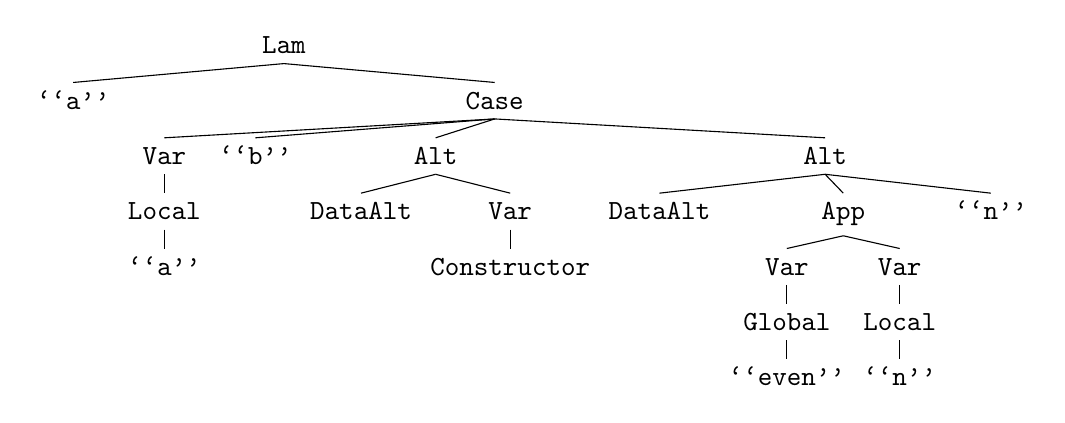
\begin{tikzpicture}[sibling distance=0pt]
        \tikzset{sibling distance=0pt}
        \tikzset{level distance=20pt}
        \Tree[ .$\CLam$
                  $\id{a}$
                  [ .$\CCase$
                       [ .$\CVar$
                            [ .$\CLocal$
                                 $\id{a}$ ]]
                       $\id{b}$
                       [ .$\CAlt$
                            $\CDataAlt$
                            [ .$\CVar$
                                 $\CConstructor$ ]]
                       [ .$\CAlt$
                            $\CDataAlt$
                            [ .$\CApp$
                                 [ .$\CVar$
                                      [ .$\CGlobal$
                                           $\id{even}$ ]]
                                 [ .$\CVar$
                                      [ .$\CLocal$
                                           $\id{n}$ ]]]
                            $\id{n}$ ]]]
      \end{tikzpicture}
    \end{small}
    \caption{AST for the \texttt{odd} function. The variable names \texttt{a}, \texttt{b}, etc.\ are chosen arbitrarily.}
    \label{fig:astexample}
\end{figure}

These recursive calls to the clustering algorithm (we use a standard
\emph{k-means} implementation) allow expressions to be compared in a
principled way: the similarity of expressions depends on the similarity of the expressions they reference, and so on recursively. In practice, this recursive
algorithm can be implemented in an iterative way, by accumulating the set of expressions to cluster in topological order of their dependency graph.

Figure~\ref{fig:astexample} shows the AST for the following Haskell function \texttt{odd}, which determines if a Peano numeral is odd:

\begin{lstlisting}[language=Haskell]
odd  Z    = False
odd (S n) = even n

even  Z    = True
even (S n) = odd n
\end{lstlisting}

The \texttt{odd} function references four global variables: \texttt{Z}, \texttt{S}, \texttt{False} and \texttt{even}. Our algorithm doesn't yet distinguish between data constructors, so the only global reference we replace is \texttt{even}. Likewise, the definition of \texttt{even} references \texttt{Z}, \texttt{S}, \texttt{True} and \texttt{odd}. For mutual recursion like this, there is no valid topological order, so we use a sentinel value as the feature.

These feature vectors are sent through a k-means clustering algorithm, using the \textsc{Weka} machine learning library. For example, the feature vector for \texttt{odd} (padded to 6 labels for each level of the tree) will begin:

\begin{equation*}
  (\feature{\CLam}, 0, 0, 0, 0, 0, \feature{\id{a}}, \feature{\CCase}, 0, 0, 0, 0, \feature{\CVar}, \feature{\id{b}}, \dots )
\end{equation*}

\section{Implementation}\label{implementation}

We obtain ASTs from Haskell projects using a bespoke plugin for the GHC
compiler. From these ASTs, we extract type information which is used to append variables to the signature; and dependency information, which is used to topologically sort the clustering rounds. We then invoke our iterative algorithm, which alternates between feature extraction and clustering until all elements of the signature have been clustered. Each cluster is converted into a \textsc{QuickSpec} signature, by extracting those functions which
\begin{inlinelist}
\item have an argument type which we can randomly generate
\item have an output type which we can compare
\end{inlinelist}. \textsc{QuickSpec} is invoked on each signature, and the resulting sets of conjectures are combined.

\section{Results}\label{results}

We have developed a machine learning approach for analysing Haskell code, including a
bespoke feature extraction method and a full implementation pipeline for turning Haskell packages into sets of equations.

\section{Difficulties and Future Work}\label{future-work}

The most difficult aspect of performing this exploration was obtaining real code in a usable format, due to the myriad edge-cases encountered. We make extensive use of Haskell's existing infrastructure, including the \textsc{GHC} compiler, the \textsc{cabal} build system, the \textsc{Hackage} code repository and the \textsc{Nix} package manager. Unfortunately, some of these systems are rather monolithic, which makes it difficult to invoke particular algorithms, such as \textsc{GHC}'s type class resolution, on their own. Whilst we have worked around these issues, e.g.\ using meta-programming, this introduces unnecessary latency, fragility and complexity.

Our investigation of recurrent clustering and theory exploration only scratches the surface of combining symbolic and statistical AI algorithms. As well as benchmarking our approach against other techniques, there are many similar opportunities to be explored, where the reasoning power of symbolic algorithms can be guided and supervised by statistical, data-driven processes.

\bibliographystyle{plain}
\bibliography{./Bibtex}

\end{document}
